%% =========================================================================
%%  NEXUS SUPPORT -- VTU Project Report (version matching
%%  "Nexus_Support_Project_Report (1).pdf")
%%
%%  Compile with:   pdflatex Nexus_Support_Project_Report_v2.tex   (run 3 times)
%%  or:             latexmk -pdf Nexus_Support_Project_Report_v2.tex
%%
%%  Optional images (put them in a "figures" folder next to this file).
%%  If an image is missing, a labeled placeholder box is drawn instead,
%%  so the document always compiles:
%%     figures/vtu_logo.png
%%     figures/karnataka_emblem.png
%%     figures/screen_ai_ready.png            (Figure 6.1)
%%     figures/screen_ai_general.png          (Figure 6.2)
%%     figures/screen_mesh_debug.png          (Figure 6.3)
%%     figures/device_emergency_bleeding.png  (Figure 6.4)
%% =========================================================================
\documentclass[12pt,a4paper]{report}

\usepackage[a4paper,top=24mm,bottom=24mm,left=24mm,right=20mm,includehead,includefoot,headheight=18pt,headsep=12pt,footskip=14pt]{geometry}
\usepackage[T1]{fontenc}
\usepackage[utf8]{inputenc}
\usepackage{mathptmx}
\usepackage[scaled=.90]{helvet}
\usepackage{courier}
\usepackage{graphicx}
\usepackage{xcolor}
\usepackage{amsmath,amssymb}
\usepackage{listings}
\usepackage{tabularx}
\usepackage{array}
\usepackage{fancyhdr}
\usepackage{eso-pic}
\usepackage{titlesec}
\usepackage{titletoc}
\usepackage{enumitem}
\usepackage[labelfont=bf]{caption}
\usepackage{adjustbox}
\usepackage{setspace}
\usepackage{url}
\urlstyle{same}
\DeclareUrlCommand\code{\urlstyle{tt}}
\usepackage{tikz}
\usetikzlibrary{calc,positioning,shapes.geometric,arrows.meta,fit,backgrounds}

\setstretch{1.12}
\setlist{itemsep=2pt,topsep=4pt,parsep=0pt}
\setlength{\parindent}{0pt}
\setlength{\parskip}{6pt}
\emergencystretch=2em

% ----------------------------------------------------------------- colors
\definecolor{vtumaroon}{RGB}{128,0,0}
\definecolor{vtublue}{RGB}{20,60,140}
\definecolor{darkslate}{RGB}{30,41,59}
\definecolor{codegray}{RGB}{245,247,250}

% ----------------------------------------------------- image with fallback
\newcommand{\safeimg}[2]{%
  \IfFileExists{#1}{\includegraphics[#2]{#1}}{%
    \fbox{\parbox[c][4cm][c]{0.6\linewidth}{\centering\scriptsize\ttfamily Missing image:\\\detokenize{#1}}}}}

% ------------------------------------------------------------ code listings
\lstset{
  backgroundcolor=\color{codegray},
  basicstyle=\ttfamily\footnotesize,
  breaklines=true,
  frame=single,
  rulecolor=\color{black!30},
  numbers=left,
  numberstyle=\tiny\color{gray},
  captionpos=b,
  keywordstyle=\bfseries\color{vtublue},
  commentstyle=\itshape\color{green!50!black},
  stringstyle=\color{vtumaroon},
  xleftmargin=1.6em,
  aboveskip=8pt,
  belowskip=4pt
}
\AtBeginDocument{\numberwithin{lstlisting}{chapter}}
\renewcommand{\lstlistingname}{Listing}

% --------------------------------------------------- page border on all pages
\AddToShipoutPictureBG{%
  \begin{tikzpicture}[remember picture, overlay]
    \draw[line width=1.5pt, color=black] ($(current page.north west)+(14mm,-14mm)$) rectangle ($(current page.south east)+(-14mm,14mm)$);
  \end{tikzpicture}%
}

% ------------------------------------------------------------ header/footer
\pagestyle{fancy}
\fancyhf{}
\fancyhead[L]{\small\textbf{\color{darkslate}NEXUS SUPPORT: EMERGENCY MESH SYSTEM}}
\fancyhead[R]{\small\textbf{\color{darkslate}2025-26}}
\fancyfoot[L]{\small\color{darkslate}Dept. of CSE, GEC, Hassan}
\fancyfoot[R]{\small\textbf{\color{darkslate}Page \thepage}}
\renewcommand{\headrule}{\color{vtumaroon}\hrule width\headwidth height 1.2pt \vskip 1pt \hrule width\headwidth height 0.4pt}
\renewcommand{\footrule}{\color{vtumaroon}\hrule width\headwidth height 0.4pt \vskip 1pt \hrule width\headwidth height 1.2pt}
\fancypagestyle{plain}{%
  \fancyhf{}
  \fancyhead[L]{\small\textbf{\color{darkslate}NEXUS SUPPORT: EMERGENCY MESH SYSTEM}}
  \fancyhead[R]{\small\textbf{\color{darkslate}2025-26}}
  \fancyfoot[L]{\small\color{darkslate}Dept. of CSE, GEC, Hassan}
  \fancyfoot[R]{\small\textbf{\color{darkslate}Page \thepage}}
  \renewcommand{\headrule}{\color{vtumaroon}\hrule width\headwidth height 1.2pt \vskip 1pt \hrule width\headwidth height 0.4pt}
  \renewcommand{\footrule}{\color{vtumaroon}\hrule width\headwidth height 0.4pt \vskip 1pt \hrule width\headwidth height 1.2pt}
}

% ----------------------------------------------------------------- headings
\titleformat{\chapter}[display]
  {\bfseries}
  {\Large Chapter \thechapter}
  {8pt}
  {\centering\LARGE}
\titlespacing*{\chapter}{0pt}{0pt}{18pt}
\titleformat{\section}{\bfseries\large}{\thesection}{0.8em}{\MakeUppercase}
\titlespacing*{\section}{0pt}{14pt}{6pt}
\titleformat{\subsection}{\bfseries\normalsize}{\thesubsection}{0.8em}{}
\titlespacing*{\subsection}{0pt}{10pt}{4pt}

% -------------------------------------------------------- contents formatting
\renewcommand{\contentsname}{TABLE OF CONTENTS}
\renewcommand{\listfigurename}{LIST OF FIGURES}
\renewcommand{\listtablename}{LIST OF TABLES}
\titlecontents{chapter}[0em]{\addvspace{6pt}\bfseries}{\contentslabel[\thecontentslabel.]{1.8em}}{}{\titlerule*[0.7pc]{.}\contentspage}
\titlecontents{section}[1.8em]{}{\contentslabel{2.4em}}{}{\titlerule*[0.7pc]{.}\contentspage}
\titlecontents{subsection}[4.2em]{}{\contentslabel{3.2em}}{}{\titlerule*[0.7pc]{.}\contentspage}
\titlecontents{figure}[0em]{}{Figure~\thecontentslabel:\quad}{}{\titlerule*[0.7pc]{.}\contentspage}
\titlecontents{table}[0em]{}{Table~\thecontentslabel:\quad}{}{\titlerule*[0.7pc]{.}\contentspage}

% ----------------------------------------------------------- reference items
\newcommand{\refitem}[2]{\par\noindent\hangindent=2.6em\hangafter=1 [#1]\hspace{0.9em}#2\par\vspace{2pt}}

% ------------------------------------------------------------ TikZ helpers
\tikzset{
  arrow/.style={-{Latex[length=2.2mm]}, thick},
  box/.style={rectangle, draw=black, fill=blue!5, thick, align=center, rounded corners, minimum height=1.0cm, font=\small},
  secbox/.style={rectangle, draw=vtumaroon, fill=red!5, thick, align=center, rounded corners, minimum height=1.0cm, font=\small}
}
\newcommand{\actor}[3]{%
  \begin{scope}[shift={(#1,#2)}]
    \draw[thick] (0,0.55) circle (0.2);
    \draw[thick] (0,0.35)--(0,-0.15) (-0.3,0.2)--(0.3,0.2) (0,-0.15)--(-0.25,-0.6) (0,-0.15)--(0.25,-0.6);
    \node[font=\small\bfseries,below] at (0,-0.6) {#3};
  \end{scope}}

\begin{document}

% =========================================================================
% TITLE PAGE
% =========================================================================
\thispagestyle{empty}
\begin{center}
  {\bfseries\large VISVESVARAYA TECHNOLOGICAL UNIVERSITY}\\[0.15cm]
  {\bfseries\normalsize ``JNANA SANGAMA'', BELAGAVI -- 590 018}\\[0.5cm]
  \safeimg{figures/vtu_logo.png}{width=2.4cm}\\[0.5cm]
  {\normalsize PROJECT REPORT ON}\\[0.3cm]
  {\bfseries\Large\color{vtublue} ``NEXUS SUPPORT: DECENTRALIZED EMERGENCY MESH COMMUNICATION AND TACTICAL INCIDENT COORDINATION PLATFORM''}\\[0.5cm]
  {\normalsize Submitted in partial fulfilment of the requirement\\for the award of the degree of}\\[0.3cm]
  {\bfseries\normalsize BACHELOR OF ENGINEERING}\\[0.1cm]
  {\bfseries\normalsize IN}\\[0.1cm]
  {\bfseries\normalsize COMPUTER SCIENCE AND ENGINEERING}\\[0.5cm]

  \textbf{\underline{Submitted By}}\\[0.25cm]
  {\color{vtublue}
  \renewcommand{\arraystretch}{1.25}
  \begin{tabular}{lcl}
    Anu V K       & : & 4GH24CS010 \\
    Chandana C D  & : & 4GH24CS029 \\
    Deekshith G   & : & 4GH24CS040 \\
    Kiran M S     & : & 4GH24CS060 \\
  \end{tabular}}\\[0.5cm]

  \textbf{\underline{Under the Guidance of}}\\[0.2cm]
  \textbf{Dr. Ranganatha S}\\
  Guide\\[0.5cm]

  \textbf{DEPARTMENT OF COMPUTER SCIENCE \& ENGINEERING}\\
  \textbf{GOVERNMENT ENGINEERING COLLEGE, HASSAN -- 573201}\\
  \textbf{2025-26}
\end{center}
\newpage

% =========================================================================
% CERTIFICATE
% =========================================================================
\thispagestyle{empty}
\begin{center}
  \textbf{\large GOVERNMENT ENGINEERING COLLEGE HASSAN -- 573 201}\\
  \small Affiliated to VTU, Belagavi \& Approved by AICTE, New Delhi\\[0.05cm]
  \textbf{\normalsize DEPARTMENT OF COMPUTER SCIENCE \& ENGINEERING}\\[0.3cm]
  \safeimg{figures/karnataka_emblem.png}{width=2.5cm}\\[0.4cm]
  \textbf{\Large CERTIFICATE}\\[0.2cm]
\end{center}

{\sloppy\setlength{\parindent}{1.5em}
Certified that the Project work entitled \textbf{``NEXUS SUPPORT: DECENTRALIZED EMERGENCY MESH COMMUNICATION AND TACTICAL INCIDENT COORDINATION PLATFORM''} carried out by \textbf{Anu V K (4GH24CS010), Chandana C D (4GH24CS029), Deekshith G (4GH24CS040) and Kiran M S (4GH24CS060)}, bonafide students of \textbf{Government Engineering College Hassan}, in partial fulfilment for the award of \textbf{Bachelor of Engineering in Computer Science and Engineering} of the \textbf{Visvesvaraya Technological University, Belagavi} during the academic year 2025-2026. It is certified that all corrections and suggestions indicated during internal evaluation have been incorporated in the report. The Project report has been approved as it satisfies the academic requirements in respect of Project work prescribed for the said Degree.\par}
\vspace{0.8cm}

\noindent
\begin{tabular}{p{7.5cm}p{7.5cm}}
\textbf{Dr. Ranganatha S} & \textbf{Dr. Vani V G}\\
Guide & Project Co-Ordinator\\[1.2cm]
\textbf{Dr. Vani V G} & \textbf{Dr. Girish D P}\\
HoD, Dept. of CSE & Principal
\end{tabular}\\[1.0cm]

\noindent
\textbf{Name of the Examiners} \hfill \textbf{Signature with Date}\\[0.4cm]
1. ..................................................... \hfill .....................................................\\[0.4cm]
2. ..................................................... \hfill .....................................................
\newpage
\ClearShipoutPictureBG

% =========================================================================
% DECLARATION
% =========================================================================
\thispagestyle{empty}
\begin{center}
  \textbf{\Large DECLARATION}\\[1.0cm]
\end{center}

{\sloppy\setlength{\parindent}{1.5em}
We, \textbf{ANU V K, CHANDANA C D, DEEKSHITH G and KIRAN M S}, students of B.E., \textbf{GOVERNMENT ENGINEERING COLLEGE, HASSAN} bearing USNs \textbf{4GH24CS010, 4GH24CS029, 4GH24CS040 and 4GH24CS060} respectively, hereby declare that the Project entitled \textbf{``NEXUS SUPPORT: DECENTRALIZED EMERGENCY MESH COMMUNICATION AND TACTICAL INCIDENT COORDINATION PLATFORM''} has been carried out by us under the supervision of our Guide, \textbf{DR. RANGANATHA S}, Department of Computer Science \& Engineering, Government Engineering College, Hassan.\par}

\vspace{0.4cm}
{\setlength{\parindent}{1.5em}
We have submitted this report in partial fulfilment of the requirements for the award of the Degree of Bachelor of Engineering in Computer Science \& Engineering by the Visvesvaraya Technological University, Belagavi during the academic year 2025-2026. This report has not been submitted to any other Organization or University for the award of any degree or certificate.\par}

\vspace{1.2cm}
\noindent
\textbf{Date:} November 20, 2026 \hfill \textbf{Project Associates:}\\[0.2cm]
\textbf{Place:} Hassan \hfill ANU V K\\
\null \hfill CHANDANA C D\\
\null \hfill DEEKSHITH G\\
\null \hfill KIRAN M S
\newpage

% =========================================================================
% ACKNOWLEDGEMENT
% =========================================================================
\pagenumbering{roman}
\setcounter{page}{1}

\begin{center}
  \textbf{\Large ACKNOWLEDGEMENT}\\[0.6cm]
\end{center}

We consider it a privilege to whole-heartedly express our gratitude and respect to each and every one who guided and helped us in the successful completion of this Project Report.

We are very thankful to the Principal, \textbf{Dr. Girish D P}, for being kind enough to provide us an opportunity to work on a project of this societal impact in this institution.

We also express our sincere gratitude to \textbf{Dr. Vani V G}, Head of the Department of Computer Science and Engineering, for her co-operation, guidance and continuous encouragement at all moments of our work.

We would like to specially mention the enthusiastic influence provided by \textbf{Dr. Ranganatha S}, Project Guide, for his invaluable ideas, critical feedback and co-operation during our venture, making this project an inspiring learning experience.

We also extend our thanks to \textbf{Dr. Vani V G}, Project Co-Ordinator, Department of Computer Science and Engineering, for the academic co-ordination and encouragement at all stages of our project work.

We would also like to thank our parents and well-wishers as well as our dear classmates for their moral support, patience and kind co-operation.

Finally, it is our pleasure to extend our appreciation to all the teaching and technical staff members of the Department of Computer Science and Engineering, GECH.

\vspace{0.8cm}
\hfill \textbf{Project Associates:}\\[0.2cm]
\null \hfill Anu V K (4GH24CS010)\\
\null \hfill Chandana C D (4GH24CS029)\\
\null \hfill Deekshith G (4GH24CS040)\\
\null \hfill Kiran M S (4GH24CS060)
\newpage

% =========================================================================
% ABSTRACT
% =========================================================================
\begin{center}
  \textbf{\Large ABSTRACT}\\[0.6cm]
\end{center}

\begin{spacing}{1.0}
During major natural catastrophes such as earthquakes, tsunamis and severe cyclonic storms, commercial cellular base stations and electrical grids are frequently incapacitated. The resulting telecommunication blackout isolates victims and leaves search-and-rescue (SAR) agencies operating without real-time situational awareness. Traditional disaster-relief systems depend on centralized internet connectivity and are therefore inoperable in air-gapped disaster zones.

This project presents \textbf{Nexus Support}, a resilient, offline-first emergency mesh communication and tactical incident coordination platform with a dual-tier topology. \textbf{Tier 1 -- Austere Field Mesh:} civilian and responder Android devices self-organize into an ad-hoc, multi-hop peer-to-peer mesh using the Google Nearby Connections API ($P2P\_CLUSTER$ strategy over BLE and Wi-Fi Direct). Life-safety distress beacons receive the highest priority (P10) and preempt lower-priority packets in bounded forwarding queues. Local storage is encrypted at rest with 256-bit AES SQLCipher using Android Keystore-backed keys, mesh payloads are protected in transit with Google Tink AEAD and ECIES hybrid cryptography, and an on-device offline AI assistant gives first-aid guidance, defended against prompt injection by strict XML prompt sandboxing.

\textbf{Tier 2 -- Tactical Operations Center:} when a field node reaches cellular, satellite or local LAN connectivity it acts as an autonomous gateway and synchronizes beacons through a transactional outbox to a FastAPI backend with PostgreSQL/PostGIS spatial indexing ($Geometry(Point, 4326)$). Incidents and responder telemetry stream over WebSockets to a React/Leaflet command dashboard that enforces a Zero-Fabrication Charter by quarantining beacons without a verified GPS fix and renders offline maps from a local HTTP tile server.

Automated verification across all tiers -- 128 backend pytest tests, 17 frontend Vitest tests and 149 Android Gradle tasks -- passed cleanly, demonstrating a secure, privacy-preserving emergency communication platform.
\end{spacing}

\vspace{0.4cm}
\noindent\textbf{Keywords:} Emergency Mesh Networking, Offline-First Architecture, Delay-Tolerant Networking (DTN), Google Nearby Connections, Google Tink, SQLCipher, PostGIS Spatial Dispatch, Zero GPS Fabrication.
\newpage

% =========================================================================
% TABLE OF CONTENTS, LIST OF FIGURES, LIST OF TABLES
% =========================================================================
\tableofcontents
\newpage
\listoffigures
\vspace{0.8cm}
\begingroup
\let\clearpage\relax
\let\cleardoublepage\relax
\listoftables
\endgroup
\newpage

% =========================================================================
% CHAPTER 1
% =========================================================================
\pagenumbering{arabic}
\setcounter{page}{1}

\chapter{INTRODUCTION}

\section{Project Overview}
Natural disasters such as flash floods, severe earthquakes, landslides and urban structural collapses routinely devastate municipal power infrastructure and cellular towers. In these scenarios, conventional communication tools -- cellular telephony, SMS, messaging applications and internet-dependent emergency hotlines -- suffer catastrophic failure. Victims trapped in disaster zones cannot call for help, and first responders cannot coordinate search-and-rescue (SAR) operations without risking life and precious time.

\textbf{Nexus Support} is an autonomous, mobile-first, decentralized emergency mesh communication and incident coordination platform. It enables smartphones to discover each other automatically, form multi-hop peer-to-peer mesh networks and route encrypted emergency distress signals (SOS) completely independent of cellular service, SIM cards or internet access.

The architecture bridges field victims, civilian volunteers, front-line search teams and centralized tactical incident commanders. As distress signals hop across neighbouring devices, gateway nodes opportunistically synchronize distress records with a geospatial command backend built on FastAPI, PostgreSQL and PostGIS. Real-time situation maps, responder tracking and dispatch downlink management are presented on a tactical operations dashboard, giving disaster-management authorities actionable situational awareness.

\section{Problem Statement}
When municipal telecommunication infrastructure is knocked offline during a sudden disaster:
\begin{enumerate}
    \item \textbf{Complete isolation:} Trapped individuals cannot broadcast emergency beacons or describe life-threatening medical conditions without cellular or Wi-Fi towers.
    \item \textbf{Uncoordinated field assets:} Responder units operate with no tactical visibility into victim coordinates, leading to redundant search efforts and tragic delays in resource allocation.
    \item \textbf{Data insecurity and fabricated telemetry:} Ad-hoc emergency systems often transmit plaintext data that can be intercepted, tampered with or used for malicious false alarms. Existing mapping tools also fabricate or default missing coordinates to the origin $(0,0)$, sending rescue teams miles off target.
    \item \textbf{Absence of tactical downlinks:} Some platforms support one-way SOS broadcasts but lack verified bidirectional channels to confirm receipt to victims and to dispatch field units with structured status updates.
\end{enumerate}
There is therefore an urgent societal need for a verified, secure, offline-first mobile mesh platform capable of reliable distress delivery, cryptographic integrity and spatial incident coordination.

\section{Scope of the Project}
The scope covers both the disconnected edge environment and the connected tactical command post, aligned with the academic project guidelines [1]:
\begin{itemize}
    \item \textbf{Mobile mesh subsystem:} An Android application (Jetpack Compose) that operates without cellular service and forms ad-hoc links with Google Nearby Connections, routing distress signals and text messages across peer hops.
    \item \textbf{Cryptographic security:} Authenticated payload encryption and signatures via Google Tink, and SQLCipher 256-bit AES full-database encryption at rest.
    \item \textbf{On-device emergency AI:} A local lightweight model with on-device retrieval-augmented generation (RAG) giving first-aid triage advice without network connectivity.
    \item \textbf{Tactical cloud backend:} A FastAPI REST and WebSocket service on PostgreSQL/PostGIS for spatial proximity queries and incident clustering.
    \item \textbf{Incident command dashboard:} A React 18 web application with Leaflet mapping, offline tile fallback, responder assignment panels and strict zero-fabrication coordinate handling.
\end{itemize}

\section{Challenges in Disaster Communications}
\begin{enumerate}
    \item \textbf{Dynamic network topology:} Nodes move, join and drop out continuously. Routing must avoid loops, broadcast storms and queue exhaustion under chaotic RF conditions.
    \item \textbf{Battery and hardware constraints:} Continuous radio scanning and cryptography drain batteries, so algorithms must have low complexity and bounded memory.
    \item \textbf{Strict zero-fabrication requirement:} Inaccurate coordinates or hallucinated telemetry can cause fatal errors; missing coordinates must never be estimated, interpolated or defaulted.
    \item \textbf{OEM Android fragmentation:} Vendors implement Wi-Fi Direct and BLE with inconsistent group negotiation and strict background-execution limits.
    \item \textbf{Prompt injection and adversarial attacks:} On-device natural-language triage must resist jailbreak prompts or injections that could alter critical medical advice.
\end{enumerate}

\section{Objectives of the Project}
\begin{itemize}
    \item To design and implement a decentralized peer-to-peer mesh engine on Android using Google Nearby Connections with autonomous multi-hop relaying.
    \item To implement a strict \textbf{Priority-10 (P10) SOS preemption engine} so that life-safety beacons jump to the head of transmission queues and evict lower-priority traffic under congestion.
    \item To protect civilian and responder privacy with Google Tink AEAD in transit and SQLCipher 256-bit AES at rest.
    \item To develop a transactional outbox mechanism providing store-and-forward, at-least-once delivery to tactical cloud gateways.
    \item To build a tactical incident command backend with FastAPI and PostgreSQL/PostGIS that runs sub-second spatial queries for nearby responders.
    \item To deliver a web-based Tactical Command Center with real-time WebSocket updates, offline raster tile caching and a strict Zero-Fabrication coordinate policy.
    \item To validate the system empirically through automated regression suites covering unit, integration and security-invariant tests.
\end{itemize}

% =========================================================================
% CHAPTER 2
% =========================================================================
\chapter{LITERATURE SURVEY}

\section{Related Works}
Emergency communication systems have evolved across several architectural paradigms.

\subsection{Centralized Cellular Public Warning Systems (PWS)}
Frameworks such as the Commercial Mobile Alert System (CMAS) and Wireless Emergency Alerts (WEA) broadcast Common Alerting Protocol (CAP) messages through cellular base stations [16]. They are effective for broad warnings before an event, but are unidirectional -- civilians cannot reply or request medical evacuation -- and stop working when base stations lose power or backhaul links are severed.

\subsection{Mobile Ad-Hoc Networks (MANETs) and Mesh Routing}
Extensive research has produced ad-hoc routing protocols such as AODV [2], Dynamic Source Routing (DSR) and Optimized Link State Routing (OLSR). Although theoretically sound, they need periodic routing-table exchanges that add control overhead and drain smartphone batteries, and they assume persistent end-to-end paths, which fails in sparse, partitioned disaster environments.

\subsection{Delay-Tolerant Networking (DTN) and Epidemic Routing}
Delay-Tolerant Networking uses a ``store-carry-and-forward'' paradigm for sparsely connected nodes [17]. In Epidemic Routing [3], nodes replicate bundles to every encountered peer, which maximises delivery probability but causes exponential duplication that exhausts memory and bandwidth. Nexus Support adopts a hybrid approach, drawing principles from Named Data and Information-Centric Networking [13]: bounded Time-To-Live (TTL) limits, message deduplication and priority-preemption queues curb broadcast storms while guaranteeing SOS delivery.

\subsection{Tactical Software Systems (ATAK and Meshtastic)}
The Android Tactical Assault Kit (ATAK), developed by the US Department of Defense, provides geospatial situational awareness using Cursor-on-Target (CoT) messages [14], but requires manual server set-up, specialised radio hardware and operator training. Meshtastic [15] offers open-source LoRa mesh communication but requires users to buy, configure and carry separate ESP32-based hardware. Nexus Support runs on commodity, unmodified Android smartphones using their built-in BLE and Wi-Fi radios with automatic, zero-configuration discovery.

\section{Comparative Analysis}

\begin{table}[htbp]
\centering
\small
\caption{Comparative Analysis of Emergency Communication Systems}
\label{tab:lit_comparison}
\renewcommand{\arraystretch}{1.3}
\begin{tabularx}{\textwidth}{|>{\raggedright\arraybackslash}p{2.5cm}|>{\raggedright\arraybackslash}X|>{\raggedright\arraybackslash}X|>{\raggedright\arraybackslash}X|>{\raggedright\arraybackslash}X|}
\hline
\textbf{Feature} & \textbf{Cellular Alerts (WEA)} & \textbf{Classic MANET (AODV)} & \textbf{Meshtastic LoRa} & \textbf{Nexus Support (Proposed)} \\
\hline
Infrastructure & Requires cell towers & Zero infrastructure & Zero (LoRa RF) & Zero infrastructure \\
\hline
Hardware & Smartphone & Smartphone & Custom LoRa dongle & Commodity smartphone \\
\hline
Bidirectional & No (broadcast only) & Yes & Yes & Yes (uplink + downlink) \\
\hline
SOS queue preemption & None & None (FIFO) & Bounded FIFO & P10 priority preemption \\
\hline
Encryption at rest & None & None & None / optional & SQLCipher 256-bit AES \\
\hline
Encryption in transit & Provider layer & Plaintext & AES-256 symmetric & Google Tink AEAD / ECIES \\
\hline
Zero GPS fabrication & N/A & Not enforced & Not enforced & Strictly quarantined \\
\hline
Spatial dispatch & None & None & None & PostgreSQL + PostGIS \\
\hline
Offline maps & N/A & None & Offline Mapbox & Vite local tile server \\
\hline
\end{tabularx}
\end{table}

% =========================================================================
% CHAPTER 3
% =========================================================================
\chapter{FEASIBILITY STUDY AND REQUIREMENTS ANALYSIS}

\section{Feasibility Study}
A systematic feasibility study confirmed that Nexus Support can be developed, verified and deployed within practical academic and real-world constraints.

\subsection{Technical Feasibility}
\begin{itemize}
    \item \textbf{Mobile layer:} Android SDK API 26+ (Android 8.0 to 14+), Kotlin 1.9+, Jetpack Compose and Google Nearby Connections, supported on the vast majority of active Android devices without rooting or custom firmware.
    \item \textbf{Cryptographic layer:} Google Tink [5] provides audited cryptographic implementations that run efficiently on ARM64 processors without a hardware security module.
    \item \textbf{Backend and spatial layer:} Python 3.11 with FastAPI for asynchronous REST/WebSocket handling, and PostgreSQL 15 with PostGIS 3.3 for high-concurrency spatial queries.
\end{itemize}
All required SDKs and libraries are accessible, actively maintained and verified through automated tests. The project is technically feasible.

\subsection{Economic Feasibility}
\begin{itemize}
    \item No commercial licenses, proprietary database fees or paid third-party cloud APIs are required; the system is built entirely on open-source frameworks.
    \item The mobile application runs on commercial off-the-shelf smartphones already owned by civilians and rescue workers.
    \item The tactical backend can be hosted on a field laptop or low-cost portable server (for example an Intel NUC or Raspberry Pi 5) on battery or solar power.
\end{itemize}
The project delivers high social and operational benefit at minimal cost and is economically feasible.

\subsection{Operational Feasibility}
\begin{itemize}
    \item A single-tap ``TRIGGER SOS'' button broadcasts a beacon immediately without technical configuration.
    \item Mesh discovery and relaying occur in the background without user intervention.
    \item The dashboard provides clear spatial markers, color-coded severity levels and automated status alerts for coordinators.
\end{itemize}
The system is operationally feasible for both untrained civilians and professional responders.

\subsection{Schedule Feasibility}
Development followed incremental, measurable milestones:
\begin{itemize}
    \item \textbf{Phase 1:} Architecture alignment, domain models and cryptographic primitives.
    \item \textbf{Phase 2:} Mesh transport, priority-queue router and Nearby Connections integration.
    \item \textbf{Phase 3:} Encrypted persistence (SQLCipher) and transactional outbox synchronization.
    \item \textbf{Phase 4:} Cloud REST/WebSocket services and PostGIS spatial dispatch.
    \item \textbf{Phase 5:} React/Leaflet command center and offline tile caching.
    \item \textbf{Phase 6:} Testing, security audit and documentation.
\end{itemize}
With comprehensive test coverage and milestone exit gates, the project was completed within the academic timeline.

\section{Functional Requirements}
\begin{enumerate}
    \item \textbf{Emergency beacon generation:} One-tap SOS capturing the current location fix (if available), distress category (medical, fire, trapped, flood) and optional notes.
    \item \textbf{Priority-preemptive mesh routing:} SOS packets are placed at priority 10, routed ahead of telemetry, and evict lower-priority packets when queues fill.
    \item \textbf{Encrypted local storage:} Message logs, node identities and beacons are encrypted at rest in a local SQLite database using SQLCipher 256-bit AES.
    \item \textbf{Transactional outbox synchronization:} When connectivity returns, background workers send stored outbox items to the cloud with idempotent delivery.
    \item \textbf{Geospatial incident ingestion:} The backend validates gateway authorisation, removes duplicates and stores coordinates as PostGIS geometry points.
    \item \textbf{Automated spatial dispatch:} Coordinators query available responders within a dynamic radius and dispatch structured assignment downlinks.
    \item \textbf{Assignment status sync-back:} Responders send \texttt{ACCEPTED} $\rightarrow$ \texttt{EN\_ROUTE} $\rightarrow$ \texttt{ON\_SCENE} $\rightarrow$ \texttt{COMPLETED} updates, validated by a strict state machine.
    \item \textbf{Offline medical triage assistant:} An on-device AI assistant answers first-aid queries from local medical guides without internet access.
\end{enumerate}

\section{Non-Functional Requirements}

\subsection{Performance Requirements}
\begin{itemize}
    \item \textbf{SOS dispatch latency:} Local queue insertion and broadcast must complete in under 50 ms on the device.
    \item \textbf{Spatial query latency:} PostGIS proximity search (\texttt{ST\_DWithin}) must run in under 10 ms for more than 10,000 incident points.
    \item \textbf{Lightweight payload:} The wire format must be compact to avoid saturating low-bandwidth radio channels.
\end{itemize}

\subsection{Safety Requirements (The Zero-Fabrication Charter)}
\begin{itemize}
    \item \textbf{Zero location fabrication:} Without an authentic GPS lock, coordinates remain strictly null and are never estimated, interpolated or replaced by $(0.0, 0.0)$.
    \item \textbf{Unmapped incident quarantining:} The dashboard places beacons without a GPS lock in an ``AWAITING GPS FIX'' drawer so teams are not sent to invalid locations.
    \item \textbf{Fail-closed security:} If database key verification fails, the database refuses decryption rather than falling back to plaintext storage.
\end{itemize}

\subsection{Security Requirements}
\begin{itemize}
    \item \textbf{Confidentiality and integrity:} In-transit packets are encrypted and authenticated using Google Tink AEAD (AES-256-GCM).
    \item \textbf{Multi-tenant isolation:} All backend queries are scoped by \texttt{organization\_id}; cross-tenant access returns HTTP 403 Forbidden.
    \item \textbf{Prompt-injection defense:} The offline AI wraps retrieved first-aid text in XML delimiter fences (\texttt{<emergency\_corpus>}) and rejects adversarial injection prompts.
\end{itemize}

\section{Hardware Requirements}

\begin{table}[htbp]
\centering
\small
\caption{Hardware Requirements}
\label{tab:hw}
\renewcommand{\arraystretch}{1.3}
\begin{tabularx}{\textwidth}{|>{\raggedright\arraybackslash}p{2.4cm}|>{\raggedright\arraybackslash}X|>{\raggedright\arraybackslash}X|}
\hline
\textbf{Component} & \textbf{Mobile client device} & \textbf{Tactical base station (gateway / server)} \\
\hline
Processor & Octa-core ARM64 (Snapdragon 600 series / MediaTek Helio or higher) & Intel Core i5 / AMD Ryzen 5 or ARM64 quad-core \\
\hline
RAM & 3 GB minimum (4 GB recommended for offline AI) & 8 GB minimum (16 GB recommended) \\
\hline
Storage & 32 GB (at least 500 MB free for encrypted DB and triage assets) & 256 GB NVMe SSD \\
\hline
Wireless / network & Bluetooth 4.2+ (BLE) and Wi-Fi 802.11 b/g/n (Wi-Fi Direct) & Gigabit Ethernet, optional Wi-Fi tactical hotspot \\
\hline
Sensors & GPS / GLONASS receiver & -- \\
\hline
\end{tabularx}
\end{table}

\section{Software Requirements}

\begin{table}[htbp]
\centering
\small
\caption{Software Requirements}
\label{tab:sw}
\renewcommand{\arraystretch}{1.3}
\begin{tabularx}{\textwidth}{|>{\raggedright\arraybackslash}p{3.6cm}|>{\raggedright\arraybackslash}X|}
\hline
\textbf{Layer} & \textbf{Specification} \\
\hline
Mobile platform & Android 8.0 (API 26) or higher; compiled against Android 14 (API 34) \\
\hline
Development environment & Android Studio Hedgehog / Iguana, JDK 21, Visual Studio Code \\
\hline
Mobile libraries & Jetpack Compose, Kotlin Coroutines and Flow, Room 2.6, SQLCipher 4.9.0, Google Nearby Connections 18.0, Google Tink 1.10 \\
\hline
Backend stack & Python 3.11+, FastAPI 0.109, Uvicorn, SQLAlchemy 2.0, Alembic 1.13, PostgreSQL 15, PostGIS 3.3 \\
\hline
Frontend stack & Node.js 18+, React 18, Vite 5, React-Leaflet 4.2, TailwindCSS 3.4 \\
\hline
\end{tabularx}
\end{table}

% =========================================================================
% CHAPTER 4
% =========================================================================
\chapter{SYSTEM DESIGN}

The system design defines the component architecture, development environments and technology frameworks used across the mobile edge tier and the tactical cloud command tier.

\section{Integrated Development Environments (IDEs)}
\begin{itemize}
    \item \textbf{Android Studio:} The primary IDE for the native Android application, providing Kotlin profiling, the Layout Inspector for Jetpack Compose, Robolectric unit-testing integration and Gradle build optimization.
    \item \textbf{Visual Studio Code:} Used for the Python FastAPI backend, SQL migration scripts, React frontend components and automated integration tests.
\end{itemize}

\section{Cloud Backend Framework (FastAPI and Uvicorn)}
FastAPI [7, 12] was chosen for the tactical backend for its performance, native asynchronous support and automatic OpenAPI schema validation. Key capabilities:
\begin{itemize}
    \item \textbf{Asynchronous throughput:} Built on Starlette and AnyIO, handling many concurrent connections during gateway offloading.
    \item \textbf{Pydantic validation:} Strict data models reject malformed distress signals and invalid coordinate types.
    \item \textbf{WebSocket hub:} Persistent low-latency duplex channels push incidents to browser clients instantly.
\end{itemize}

\section{Database Architecture and PostGIS Spatial Engine}
The persistence layer couples the SQLAlchemy 2.0 ORM with PostgreSQL 15 and the PostGIS extension [8]. Incidents and responder positions are stored as native points in spatial reference system 4326 (WGS 84):
\begin{equation}
    \text{location} = \text{ST\_SetSRID}\bigl(\text{ST\_MakePoint}(\text{longitude}, \text{latitude}),\, 4326\bigr)
\end{equation}
Generalized Search Tree (GiST) indexes enable sub-millisecond proximity queries, for example finding available responders within 5 km of a point:
\begin{lstlisting}[language=SQL,caption={PostGIS Proximity Query}]
SELECT id, callsign,
       ST_Distance(location, ST_MakePoint(-122.419, 37.775)::geography)
FROM responders
WHERE ST_DWithin(location, ST_MakePoint(-122.419, 37.775)::geography, 5000)
  AND status = 'AVAILABLE';
\end{lstlisting}
Database migrations are managed with versioned Alembic scripts to preserve schema integrity (current migration head: \texttt{6f1a8b92c431}).

\section{Mobile Client Architecture (Jetpack Compose and Room)}
The Android application follows Clean Architecture principles:
\begin{itemize}
    \item \textbf{Jetpack Compose} [10]: a declarative UI toolkit that removes legacy XML layouts and gives smooth rendering with a unified dark tactical style.
    \item \textbf{SQLCipher 4.9.0 with Room:} Room compiles SQL queries to verified bytecode, while SQLCipher [6] transparently encrypts the whole database file with 256-bit AES (CBC mode with per-page HMAC).
    \item \textbf{Android WorkManager} [11]: runs the \texttt{GatewaySyncWorker} in the background, ensuring reliable execution even if the app is closed or memory is reclaimed.
\end{itemize}

\section{Cryptographic Subsystem (Google Tink)}
\begin{itemize}
    \item \textbf{Envelope encryption:} Payloads are encrypted with symmetric keys using AES-256-GCM [19].
    \item \textbf{Asymmetric key encapsulation:} Public-key operations use the Elliptic Curve Integrated Encryption Scheme (ECIES) with HKDF-SHA256 key derivation.
    \item \textbf{Hardware key protection:} Private keys and the master database passphrase are sealed in the hardware-backed Android Keystore.
\end{itemize}

\section{Tactical Web Dashboard (React 18 and Leaflet)}
\begin{itemize}
    \item \textbf{React 18 and Vite:} a fast, modular client with instant hot-module replacement and a production bundle under 360 kB.
    \item \textbf{React-Leaflet:} open-source interactive mapping with multiple raster layers (RF Mesh, OpenTopoMap, Satellite) [9].
    \item \textbf{Offline tile fallback:} a local raster tile HTTP server can be configured with HOT [20] exports through \code{VITE_LOCAL_TILE_URL} so maps render without internet.
\end{itemize}

% =========================================================================
% CHAPTER 5
% =========================================================================
\chapter{SYSTEM ARCHITECTURE}

\section{System Architecture Overview}
Nexus Support bridges edge field communications with tactical command operations across two complementary tiers, as shown in Figure~\ref{fig:sys_arch}. In Tier~1, victim, relay, gateway and responder phones form an offline mesh. In Tier~2, a gateway node uploads beacons over HTTPS (authenticated by the \texttt{X-Gateway-Key} header) to the FastAPI backend, which stores them in PostgreSQL/PostGIS and streams them to the tactical web map; dispatch downlinks travel back along the same path, following classical end-to-end design principles in distributed networks [18].

\begin{figure}[htbp]
\centering
\begin{adjustbox}{max width=\linewidth}
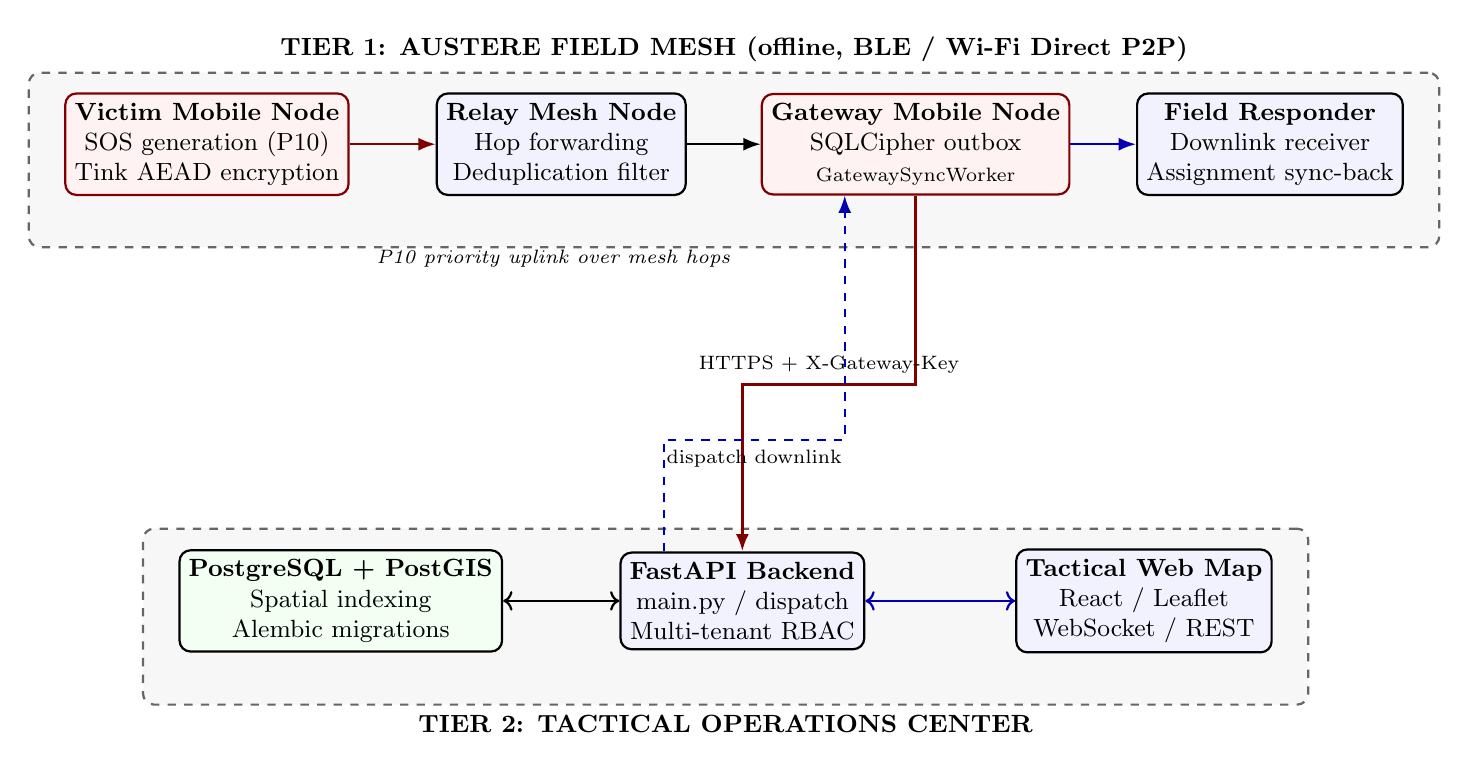
\begin{tikzpicture}[font=\footnotesize]
  % Tier 1
  \node[secbox] (victim) at (0,0) {\textbf{Victim Mobile Node}\\SOS generation (P10)\\Tink AEAD encryption};
  \node[box] (relay) at (4.5,0) {\textbf{Relay Mesh Node}\\Hop forwarding\\Deduplication filter};
  \node[secbox] (gateway) at (9.0,0) {\textbf{Gateway Mobile Node}\\SQLCipher outbox\\\scriptsize GatewaySyncWorker};
  \node[box] (responder) at (13.5,0) {\textbf{Field Responder}\\Downlink receiver\\Assignment sync-back};
  \draw[arrow, color=vtumaroon] (victim) -- (relay);
  \draw[arrow] (relay) -- (gateway);
  \draw[arrow, color=blue!70!black] (gateway) -- (responder);
  \node[font=\scriptsize\itshape] at (4.4,-1.45) {P10 priority uplink over mesh hops};
  \begin{scope}[on background layer]
    \node[draw=black!60, dashed, thick, rounded corners, fill=gray!6, fit=(victim)(relay)(gateway)(responder), inner sep=0.45cm, yshift=-0.2cm,
          label={[font=\small\bfseries]above:TIER 1: AUSTERE FIELD MESH (offline, BLE / Wi-Fi Direct P2P)}] (tier1) {};
  \end{scope}
  % Tier 2
  \node[box, fill=green!5] (pg) at (1.7,-5.8) {\textbf{PostgreSQL + PostGIS}\\Spatial indexing\\Alembic migrations};
  \node[box] (api) at (6.8,-5.8) {\textbf{FastAPI Backend}\\main.py / dispatch\\Multi-tenant RBAC};
  \node[box] (web) at (11.9,-5.8) {\textbf{Tactical Web Map}\\React / Leaflet\\WebSocket / REST};
  \draw[arrow, <->] (pg) -- (api);
  \draw[arrow, <->, color=blue!70!black] (api) -- (web);
  \begin{scope}[on background layer]
    \node[draw=black!60, dashed, thick, rounded corners, fill=gray!6, fit=(pg)(api)(web), inner sep=0.45cm, yshift=-0.2cm,
          label={[font=\small\bfseries]below:TIER 2: TACTICAL OPERATIONS CENTER}] (tier2) {};
  \end{scope}
  % Gateway -> backend
  \draw[arrow, color=vtumaroon, line width=1.2pt] (gateway.south) -- ([yshift=-2.4cm]gateway.south) -- node[above,font=\scriptsize,text=black]{HTTPS + X-Gateway-Key} ([yshift=-2.4cm]gateway.south -| api.north) -- (api.north);
  \draw[arrow, color=blue!70!black, dashed] ([xshift=-1.0cm]api.north) -- ([xshift=-1.0cm,yshift=-3.1cm]gateway.south -| api.north) -- node[below,font=\scriptsize,text=black]{dispatch downlink} ([xshift=-0.9cm,yshift=-3.1cm]gateway.south) -- ([xshift=-0.9cm]gateway.south);
\end{tikzpicture}
\end{adjustbox}
\caption{System Architecture of Nexus Support}
\label{fig:sys_arch}
\end{figure}

\section{Mesh Packet Specification and Transports}
All wireless peer communication is encapsulated in structured \texttt{MeshPacket} containers [4]:
\begin{lstlisting}[language=Java,caption={MeshPacket Data Class}]
data class MeshPacket(
    val packetId: String = UUID.randomUUID().toString(),
    val senderId: String,
    val recipientId: String,   // "BROADCAST_ALL" or target device ID
    val priority: Int,         // 10 (SOS), 5 (Chat), 1 (Telemetry)
    val ttl: Int = 5,          // Time-to-live hop counter
    val timestamp: Long = System.currentTimeMillis(),
    val payloadType: String,   // "SOS", "CHAT", "DOWNLINK", "STATUS"
    val encryptedPayload: ByteArray,
    val signature: ByteArray
)
\end{lstlisting}

\section{Data Pre-processing and Priority Routing Engine}
In \texttt{core/mesh/.../MeshRouter.kt}, packets pass through a priority-preemptive state machine (Figure~\ref{fig:flow}):
\begin{enumerate}
    \item \textbf{Deduplication check:} If the \texttt{packetId} exists in the 5,000-entry in-memory LRU deduplication cache, the packet is silently discarded.
    \item \textbf{Hop-counter decrement:} If $TTL \le 1$ the packet has reached its maximum radius and is not forwarded; otherwise $TTL = TTL - 1$.
    \item \textbf{P10 priority insertion:} Packets enter a bounded priority queue. When the queue length reaches 50 items, an incoming SOS (priority 10) evicts the oldest non-emergency packet (priority $< 10$) to create space, while an incoming packet with priority $< 10$ is dropped.
\end{enumerate}

\begin{figure}[htbp]
\centering
\begin{adjustbox}{max width=0.95\linewidth,max height=0.55\textheight}
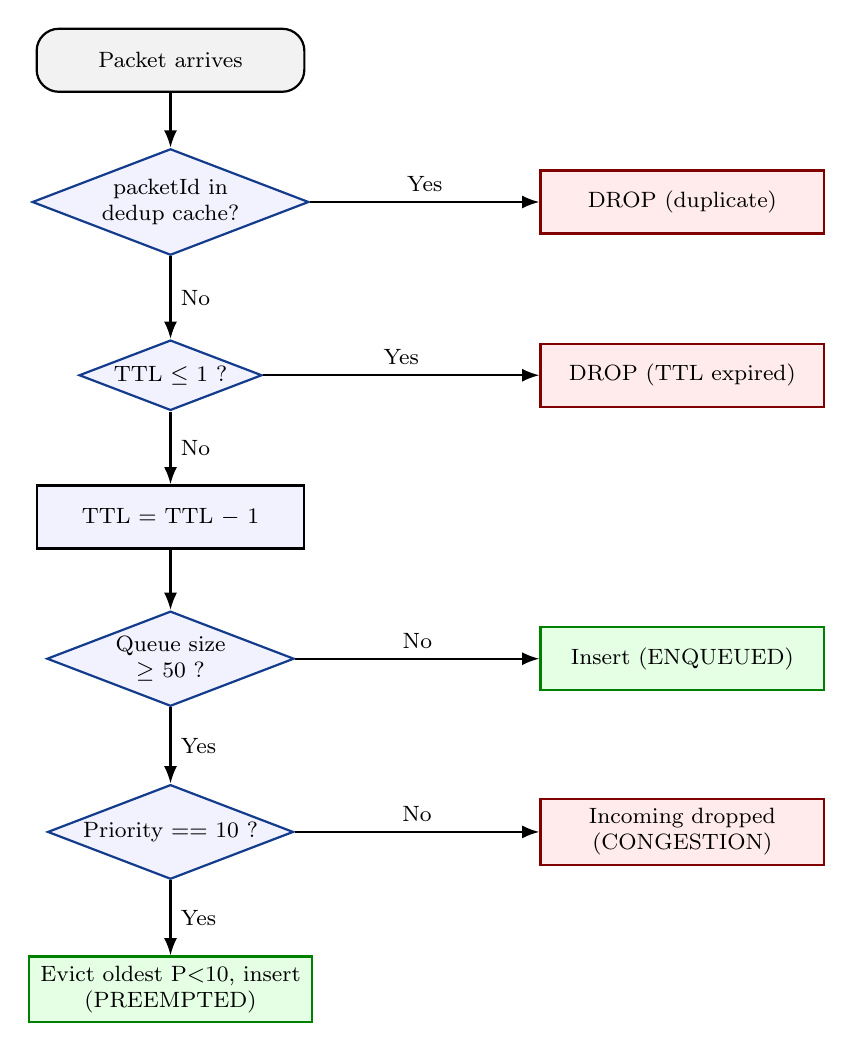
\begin{tikzpicture}[
    font=\footnotesize,
    term/.style={rectangle, rounded corners=8pt, draw=black, fill=gray!10, thick, minimum width=3.4cm, minimum height=0.8cm, align=center},
    dec/.style={diamond, aspect=2.6, draw=vtublue, fill=blue!5, thick, inner sep=1pt, align=center},
    proc/.style={rectangle, draw=black, fill=blue!5, thick, minimum width=3.4cm, minimum height=0.8cm, align=center},
    drop/.style={rectangle, draw=vtumaroon, fill=red!8, thick, minimum width=3.6cm, minimum height=0.8cm, align=center},
    ok/.style={rectangle, draw=green!50!black, fill=green!10, thick, minimum width=3.6cm, minimum height=0.8cm, align=center}
]
  \node[term] (start) at (0,0) {Packet arrives};
  \node[dec] (d1) at (0,-1.8) {packetId in\\dedup cache?};
  \node[drop] (x1) at (6.5,-1.8) {DROP (duplicate)};
  \node[dec] (d2) at (0,-4.0) {TTL $\le$ 1 ?};
  \node[drop] (x2) at (6.5,-4.0) {DROP (TTL expired)};
  \node[proc] (a1) at (0,-5.8) {TTL = TTL $-$ 1};
  \node[dec] (d3) at (0,-7.6) {Queue size\\$\ge$ 50 ?};
  \node[ok] (ok1) at (6.5,-7.6) {Insert (ENQUEUED)};
  \node[dec] (d4) at (0,-9.8) {Priority == 10 ?};
  \node[drop] (x3) at (6.5,-9.8) {Incoming dropped\\(CONGESTION)};
  \node[ok] (ok2) at (0,-11.8) {Evict oldest P$<$10, insert\\(PREEMPTED)};
  \draw[arrow] (start) -- (d1);
  \draw[arrow] (d1) -- node[right]{No} (d2);
  \draw[arrow] (d1) -- node[above]{Yes} (x1);
  \draw[arrow] (d2) -- node[right]{No} (a1);
  \draw[arrow] (d2) -- node[above]{Yes} (x2);
  \draw[arrow] (a1) -- (d3);
  \draw[arrow] (d3) -- node[above]{No} (ok1);
  \draw[arrow] (d3) -- node[right]{Yes} (d4);
  \draw[arrow] (d4) -- node[above]{No} (x3);
  \draw[arrow] (d4) -- node[right]{Yes} (ok2);
\end{tikzpicture}
\end{adjustbox}
\caption{MeshRouter Priority-Preemption Flowchart}
\label{fig:flow}
\end{figure}

\section{Use Case View}
Figure~\ref{fig:use_case} shows the primary actors and their interactions: victims trigger SOS and consult offline triage; responders receive dispatch downlinks and sync assignment status; commanders view the spatial incident map and dispatch.

\begin{figure}[htbp]
\centering
\begin{adjustbox}{max width=\linewidth}
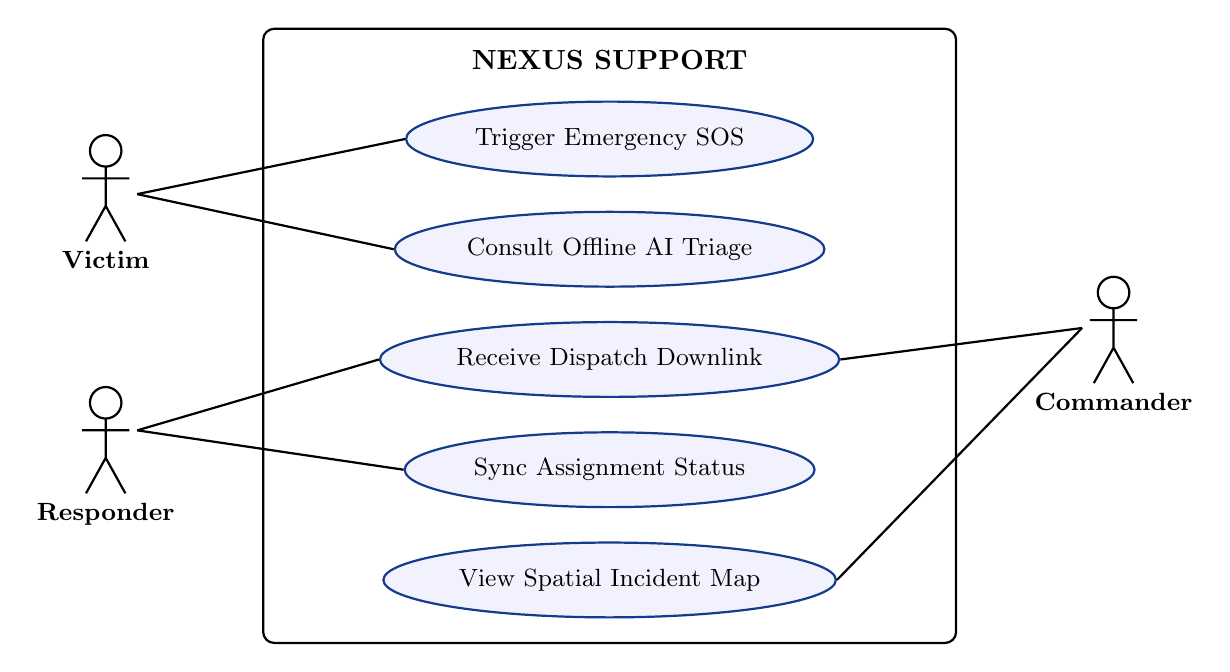
\begin{tikzpicture}[font=\small]
  \draw[thick, rounded corners=4pt] (2.6,-2.1) rectangle (11.4,5.7);
  \node[font=\bfseries] at (7,5.3) {NEXUS SUPPORT};
  \actor{0.6}{3.6}{Victim}
  \actor{0.6}{0.4}{Responder}
  \actor{13.4}{1.8}{Commander}
  \node[ellipse,draw=vtublue,fill=blue!5,thick,minimum width=5cm,minimum height=0.95cm] (uc1) at (7,4.3) {Trigger Emergency SOS};
  \node[ellipse,draw=vtublue,fill=blue!5,thick,minimum width=5cm,minimum height=0.95cm] (uc2) at (7,2.9) {Consult Offline AI Triage};
  \node[ellipse,draw=vtublue,fill=blue!5,thick,minimum width=5cm,minimum height=0.95cm] (uc3) at (7,1.5) {Receive Dispatch Downlink};
  \node[ellipse,draw=vtublue,fill=blue!5,thick,minimum width=5cm,minimum height=0.95cm] (uc4) at (7,0.1) {Sync Assignment Status};
  \node[ellipse,draw=vtublue,fill=blue!5,thick,minimum width=5cm,minimum height=0.95cm] (uc5) at (7,-1.3) {View Spatial Incident Map};
  \draw[thick] (1.0,3.6)--(uc1.west);
  \draw[thick] (1.0,3.6)--(uc2.west);
  \draw[thick] (1.0,0.6)--(uc3.west);
  \draw[thick] (1.0,0.6)--(uc4.west);
  \draw[thick] (13.0,1.9)--(uc5.east);
  \draw[thick] (13.0,1.9)--(uc3.east);
\end{tikzpicture}
\end{adjustbox}
\caption{System Use Case Diagram}
\label{fig:use_case}
\end{figure}

\section{Data Flow Diagrams}

\subsection{DFD Level 0 (Context Diagram)}
The context diagram shows Nexus Support as one process between field victims/responders and the tactical command center, exchanging distress signals, downlink dispatches, actionable telemetry and dispatch operations.

\begin{figure}[htbp]
\centering
\begin{adjustbox}{max width=\linewidth}
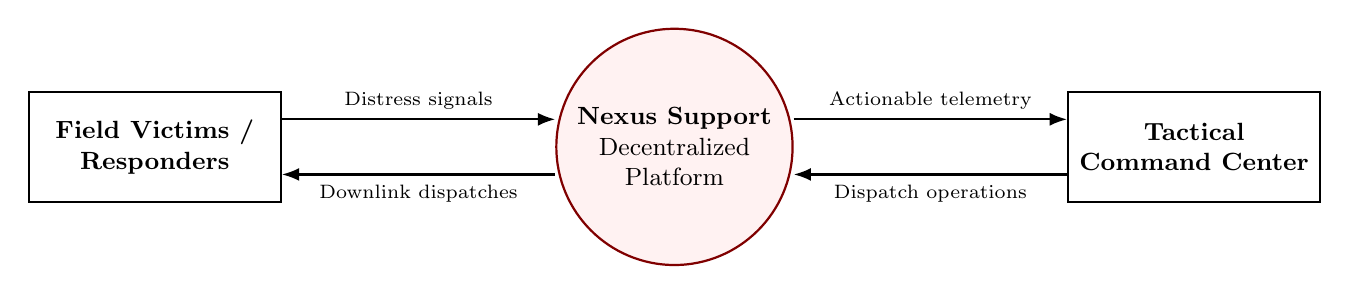
\begin{tikzpicture}[font=\small]
  \node[rectangle, draw=black, thick, minimum width=3.2cm, minimum height=1.4cm, align=center] (in) at (0,0) {\textbf{Field Victims /}\\\textbf{Responders}};
  \node[circle, draw=vtumaroon, fill=red!5, thick, minimum size=3cm, align=center] (sys) at (6.6,0) {\textbf{Nexus Support}\\Decentralized\\Platform};
  \node[rectangle, draw=black, thick, minimum width=3.2cm, minimum height=1.4cm, align=center] (out) at (13.2,0) {\textbf{Tactical}\\\textbf{Command Center}};
  \draw[arrow] ([yshift=0.35cm]in.east) -- node[above,font=\scriptsize]{Distress signals} ([yshift=0.35cm]sys.west |- in.east);
  \draw[arrow] ([yshift=-0.35cm]sys.west |- in.east) -- node[below,font=\scriptsize]{Downlink dispatches} ([yshift=-0.35cm]in.east);
  \draw[arrow] ([yshift=0.35cm]sys.east |- out.west) -- node[above,font=\scriptsize]{Actionable telemetry} ([yshift=0.35cm]out.west);
  \draw[arrow] ([yshift=-0.35cm]out.west) -- node[below,font=\scriptsize]{Dispatch operations} ([yshift=-0.35cm]sys.east |- out.west);
\end{tikzpicture}
\end{adjustbox}
\caption{Data Flow Diagram: DFD Level 0}
\label{fig:dfd_level0}
\end{figure}

\subsection{DFD Level 1}
Level~1 breaks the system into four processes -- SOS input, priority mesh routing, gateway synchronization, and tactical command map and dispatch -- with two data stores: the SQLCipher outbox (D1) and the PostGIS database (D2).

\begin{figure}[htbp]
\centering
\begin{adjustbox}{max width=\linewidth}
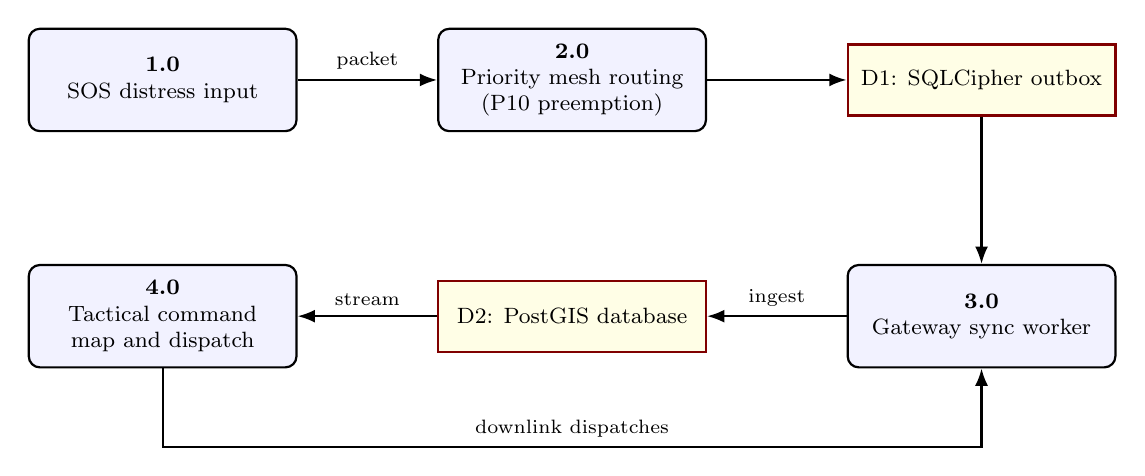
\begin{tikzpicture}[
    font=\footnotesize,
    proc/.style={rectangle, draw=black, fill=blue!5, rounded corners, thick, minimum width=3.4cm, minimum height=1.3cm, align=center},
    store/.style={rectangle, draw=vtumaroon, fill=yellow!10, thick, minimum width=3.4cm, minimum height=0.9cm, align=center}
]
  \node[proc] (p1) at (0,0) {\textbf{1.0}\\SOS distress input};
  \node[proc] (p2) at (5.2,0) {\textbf{2.0}\\Priority mesh routing\\(P10 preemption)};
  \node[store] (s1) at (10.4,0) {D1: SQLCipher outbox};
  \node[proc] (p3) at (10.4,-3) {\textbf{3.0}\\Gateway sync worker};
  \node[store] (s2) at (5.2,-3) {D2: PostGIS database};
  \node[proc] (p4) at (0,-3) {\textbf{4.0}\\Tactical command\\map and dispatch};
  \draw[arrow] (p1) -- node[above,font=\scriptsize]{packet} (p2);
  \draw[arrow] (p2) -- (s1);
  \draw[arrow] (s1) -- (p3);
  \draw[arrow] (p3) -- node[above,font=\scriptsize]{ingest} (s2);
  \draw[arrow] (s2) -- node[above,font=\scriptsize]{stream} (p4);
  \draw[arrow] (p4.south) -- ++(0,-1.0) -| node[pos=0.25,above,font=\scriptsize]{downlink dispatches} (p3.south);
\end{tikzpicture}
\end{adjustbox}
\caption{Data Flow Diagram: DFD Level 1}
\label{fig:dfd_level1}
\end{figure}

\section{Verification and Incident Lifecycle Workflows}

\subsection{Verification Workflow}
Each code tier is verified independently, followed by an end-to-end demo test covering the full incident lifecycle (Figure~\ref{fig:verify_workflow}).

\begin{figure}[htbp]
\centering
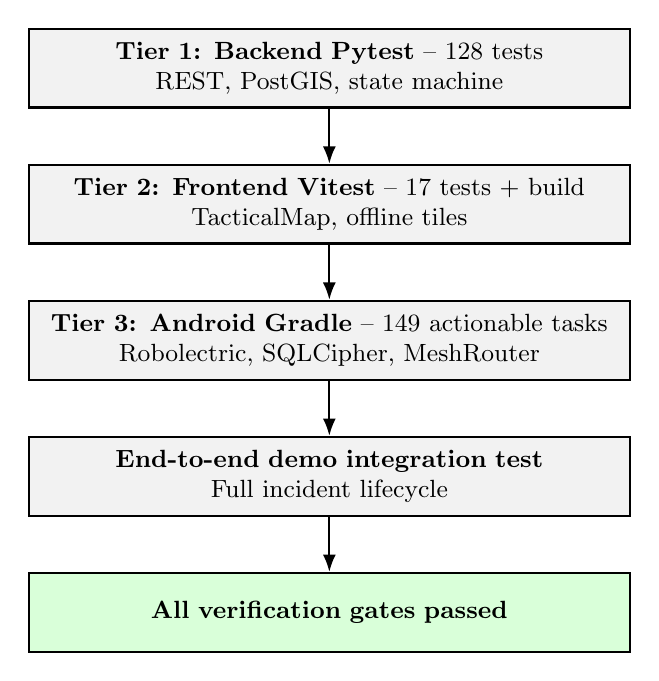
\begin{tikzpicture}[
    node distance=0.7cm,
    wstep/.style={rectangle, draw=black, fill=gray!10, thick, text width=7.4cm, align=center, minimum height=1.0cm, font=\small},
    arrow/.style={-{Latex[length=2.2mm]}, thick}
]
  \node[wstep] (w1) {\textbf{Tier 1: Backend Pytest} -- 128 tests\\REST, PostGIS, state machine};
  \node[wstep, below=of w1] (w2) {\textbf{Tier 2: Frontend Vitest} -- 17 tests + build\\TacticalMap, offline tiles};
  \node[wstep, below=of w2] (w3) {\textbf{Tier 3: Android Gradle} -- 149 actionable tasks\\Robolectric, SQLCipher, MeshRouter};
  \node[wstep, below=of w3] (w4) {\textbf{End-to-end demo integration test}\\Full incident lifecycle};
  \node[wstep, below=of w4, fill=green!15] (w5) {\textbf{All verification gates passed}};
  \draw[arrow] (w1) -- (w2);
  \draw[arrow] (w2) -- (w3);
  \draw[arrow] (w3) -- (w4);
  \draw[arrow] (w4) -- (w5);
\end{tikzpicture}
\caption{Automated Verification Workflow}
\label{fig:verify_workflow}
\end{figure}

\subsection{Incident and Assignment Lifecycle Workflow}
Responder assignments follow a finite state machine enforced by the backend (Figure~\ref{fig:fsm_workflow}). Illegal transitions are rejected, and on completion the responder is released back to \texttt{AVAILABLE}.

\begin{figure}[htbp]
\centering
\begin{adjustbox}{max width=\linewidth}
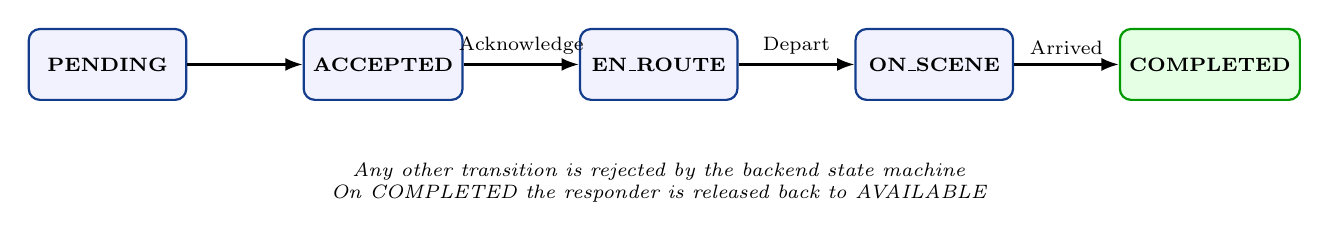
\begin{tikzpicture}[
    st/.style={rectangle, draw=vtublue, fill=blue!5, thick, rounded corners, minimum width=2.0cm, minimum height=0.9cm, font=\scriptsize\bfseries},
    trm/.style={rectangle, draw=green!60!black, fill=green!10, thick, rounded corners, minimum width=2.0cm, minimum height=0.9cm, font=\scriptsize\bfseries}
]
  \node[st] (s1) at (0,0) {PENDING};
  \node[st] (s2) at (3.5,0) {ACCEPTED};
  \node[st] (s3) at (7.0,0) {EN\_ROUTE};
  \node[st] (s4) at (10.5,0) {ON\_SCENE};
  \node[trm] (s5) at (14.0,0) {COMPLETED};
  \draw[arrow] (s1) -- (s2);
  \draw[arrow] (s2) -- node[above,font=\scriptsize]{Acknowledge} (s3);
  \draw[arrow] (s3) -- node[above,font=\scriptsize]{Depart} (s4);
  \draw[arrow] (s4) -- node[above,font=\scriptsize]{Arrived} (s5);
  \node[font=\scriptsize] at (1.75,0.3) {};
  \node[font=\scriptsize\itshape, align=center] at (7,-1.5) {Any other transition is rejected by the backend state machine\\On COMPLETED the responder is released back to AVAILABLE};
\end{tikzpicture}
\end{adjustbox}
\caption{Assignment State Transition Finite State Machine}
\label{fig:fsm_workflow}
\end{figure}

\section{Cryptographic Envelope Architecture}
In-transit packets are sealed with a two-layer cryptographic envelope (Figure~\ref{fig:crypto}):
\begin{enumerate}
    \item \textbf{Payload encryption:} The plaintext $M$ is encrypted under an ephemeral symmetric key $K_{sym}$ with AES-256-GCM, yielding ciphertext $C$ and authentication tag $T$:
    \begin{equation}
        (C, T) = \text{AES-GCM-Encrypt}(K_{sym}, \text{Nonce}, M, \text{AssociatedData})
    \end{equation}
    \item \textbf{Key encapsulation:} $K_{sym}$ is encrypted with the recipient's public elliptic-curve key using ECIES with HKDF:
    \begin{equation}
        C_{key} = \text{ECIES-Encrypt}(PK_{recipient}, K_{sym})
    \end{equation}
    \item \textbf{Integrity signature:} The sender's private Ed25519 key signs the hash of $(C \parallel T \parallel C_{key})$, providing non-repudiation.
\end{enumerate}

\begin{figure}[htbp]
\centering
\begin{adjustbox}{max width=\linewidth}
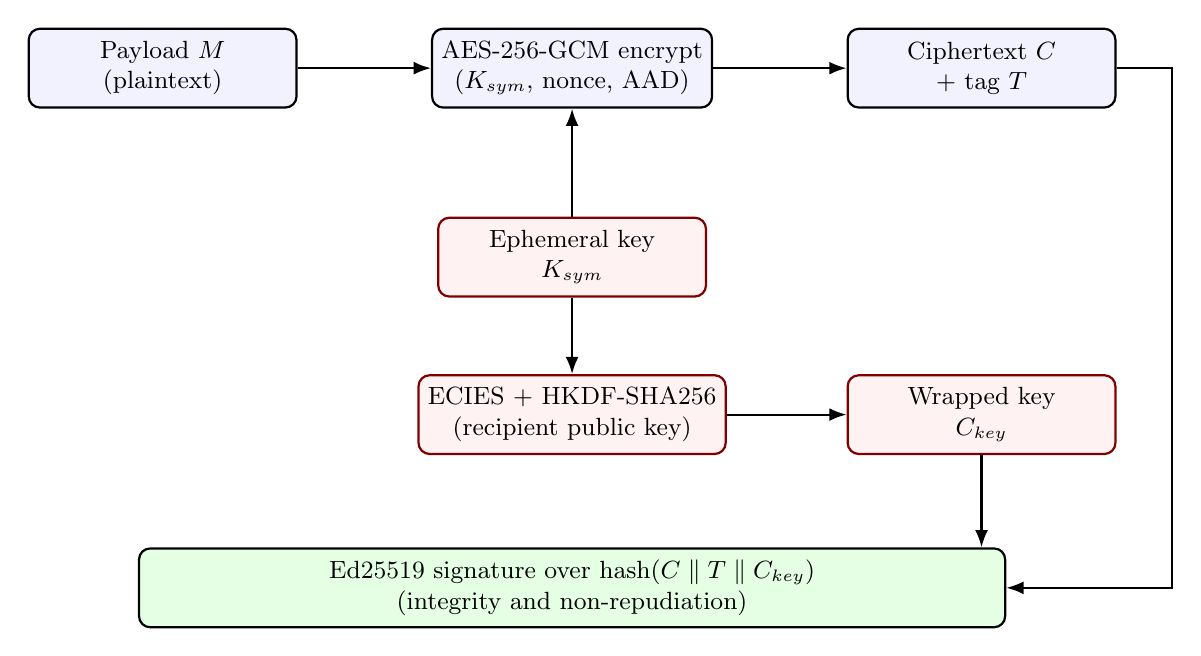
\begin{tikzpicture}[
    font=\small,
    blk/.style={rectangle, draw=black, fill=blue!5, thick, rounded corners, align=center, minimum width=3.4cm, minimum height=1.0cm},
    key/.style={rectangle, draw=vtumaroon, fill=red!5, thick, rounded corners, align=center, minimum width=3.4cm, minimum height=1.0cm}
]
  \node[blk] (m) at (0,0) {Payload $M$\\(plaintext)};
  \node[blk] (aes) at (5.2,0) {AES-256-GCM encrypt\\$(K_{sym}$, nonce, AAD$)$};
  \node[blk] (ct) at (10.4,0) {Ciphertext $C$\\+ tag $T$};
  \node[key] (k) at (5.2,-2.4) {Ephemeral key\\$K_{sym}$};
  \node[key] (ecies) at (5.2,-4.4) {ECIES + HKDF-SHA256\\(recipient public key)};
  \node[key] (ck) at (10.4,-4.4) {Wrapped key\\$C_{key}$};
  \node[rectangle, draw=black, fill=green!10, thick, rounded corners, align=center, minimum width=11cm, minimum height=1.0cm] (sig) at (5.2,-6.6) {Ed25519 signature over hash$(C \parallel T \parallel C_{key})$\\(integrity and non-repudiation)};
  \draw[arrow] (m) -- (aes);
  \draw[arrow] (aes) -- (ct);
  \draw[arrow] (k) -- (aes);
  \draw[arrow] (k) -- (ecies);
  \draw[arrow] (ecies) -- (ck);
  \draw[arrow] (ck) -- (ck |- sig.north);
  \draw[arrow] (ct.east) -- ++(0.7,0) |- (sig.east);
\end{tikzpicture}
\end{adjustbox}
\caption{Cryptographic Envelope Architecture}
\label{fig:crypto}
\end{figure}

% =========================================================================
% CHAPTER 6
% =========================================================================
\chapter{IMPLEMENTATION}

\section{Core Algorithms and Pseudo-Code}

\subsection{Priority-Preemptive Mesh Forwarding (MeshRouter)}
Algorithm 6.1 implements the safety-critical priority-preemption logic of \texttt{MeshRouter.kt}.

\begin{lstlisting}[language=Java,caption={Algorithm 6.1 -- MeshRouter Priority Preemption}]
BEGIN
1. FUNCTION EnqueuePacket(packet):
    // Check duplication cache
    IF DeduplicationCache.contains(packet.id) THEN RETURN DROP_DUPLICATE
    DeduplicationCache.add(packet.id)

    // Check hop limit
    IF packet.ttl <= 1 THEN RETURN DROP_TTL_EXPIRED
    packet.ttl = packet.ttl - 1

    // Evaluate priority-queue capacity
    IF PriorityQueue.size >= MAX_QUEUE_CAPACITY THEN
        IF packet.priority == 10 THEN      // SOS distress
            lowest = FindOldestWithPriorityLessThan(10)
            IF lowest != NULL THEN
                PriorityQueue.remove(lowest)
                PriorityQueue.insert(packet)
                RETURN SUCCESS_PREEMPTED
            ELSE RETURN DROP_QUEUE_SATURATED
            ENDIF
        ELSE RETURN DROP_CONGESTION
        ENDIF
    ELSE
        PriorityQueue.insert(packet)
        RETURN SUCCESS_ENQUEUED
    ENDIF
END
\end{lstlisting}

\subsection{Transactional Outbox Synchronization (GatewaySyncWorker)}
Algorithm 6.2 outlines the store-and-forward outbox synchronization executed by Android WorkManager. Items are marked synced only after the server acknowledges them, giving at-least-once delivery; a 403 response stops the worker because retrying cannot fix an unauthorised key.

\begin{lstlisting}[language=Java,caption={Algorithm 6.2 -- Transactional Outbox Store-and-Forward}]
BEGIN
1. FUNCTION DoWork():
    pendingItems = OutboxDao.getUnsyncedItems(limit = 20)
    IF pendingItems.isEmpty() THEN RETURN Result.success()

    FOR item IN pendingItems DO
        TRY:
            response = RetrofitClient.postSyncSos(
                gatewayKey = BuildConfig.GATEWAY_KEY,
                payload    = item.serializedPayload)
            IF response.isSuccessful() THEN
                OutboxDao.markSynced(item.id, System.currentTimeMillis())
            ELSE IF response.code() == 403 THEN
                LOG_FATAL("Gateway Key Unauthorized")
                RETURN Result.failure()
            ELSE
                RETURN Result.retry()      // bounded exponential backoff
            ENDIF
        CATCH NetworkException:
            RETURN Result.retry()
    ENDFOR
    RETURN Result.success()
END
\end{lstlisting}

\section{General Working of the System}
\begin{enumerate}
    \item \textbf{Distress trigger:} A civilian taps the large red ``TRIGGER SOS'' button. The app samples available GPS coordinates (keeping null if unacquired), packages the payload and signs it.
    \item \textbf{Ad-hoc relaying:} The packet is broadcast over Bluetooth Low Energy and Wi-Fi Direct. Intermediate devices forward it across multiple hops, prioritising it ahead of routine chat.
    \item \textbf{Gateway ingestion:} When the packet reaches a device with cellular or tactical LAN connectivity, \texttt{GatewaySyncWorker.kt} uploads it over HTTPS with the \texttt{X-Gateway-Key} header.
    \item \textbf{Spatial indexing and WebSocket stream:} The FastAPI backend saves the incident to PostgreSQL as a PostGIS point and broadcasts an alert over WebSockets to all connected consoles.
    \item \textbf{Tactical dispatch:} The commander views the beacon on \texttt{TacticalMap.jsx}, clicks ``DISPATCH REINFORCEMENTS'' and assigns a nearby responder.
    \item \textbf{Downlink receipt and status sync:} The responder receives a high-importance notification, accepts the assignment and syncs status updates back to the operations center as work progresses.
\end{enumerate}

\section{Mobile Client Implementation and Application Screens}
The mobile interface was built with Jetpack Compose following strict tactical dark-mode guidelines. The main screens are:
\begin{itemize}
    \item \textbf{Home screen:} active mesh peer connections, gateway sync state, rapid SOS trigger and shortcuts to offline triage guides.
    \item \textbf{Emergency SOS broadcast:} real-time broadcast status, hop transmission counter, verified GPS fix and distress-cancellation controls.
    \item \textbf{Offline AI assistant:} an on-device generative assistant that answers emergency queries with local model execution, with a persistent banner reminding users that responses are AI-generated and must be verified (Figures~\ref{fig:screen_ai}, \ref{fig:screen_general} and \ref{fig:screen_bleeding}).
    \item \textbf{Mesh debug dashboard:} shows the deduplicated-events cache size and the current vector-clock matrix for diagnosing mesh behavior (Figure~\ref{fig:screen_mesh}).
\end{itemize}

\begin{figure}[htbp]
\centering
\begin{minipage}[t]{0.48\textwidth}
  \centering
  \safeimg{figures/screen_ai_ready.png}{height=9.5cm,keepaspectratio}
  \captionof{figure}{Offline AI Assistant (ready state)}
  \label{fig:screen_ai}
\end{minipage}\hfill
\begin{minipage}[t]{0.48\textwidth}
  \centering
  \safeimg{figures/screen_ai_general.png}{height=9.5cm,keepaspectratio}
  \captionof{figure}{Offline AI Assistant answering a general query}
  \label{fig:screen_general}
\end{minipage}
\end{figure}

\begin{figure}[htbp]
\centering
\begin{minipage}[t]{0.48\textwidth}
  \centering
  \safeimg{figures/screen_mesh_debug.png}{height=9.5cm,keepaspectratio}
  \captionof{figure}{Mesh Debug Dashboard}
  \label{fig:screen_mesh}
\end{minipage}\hfill
\begin{minipage}[t]{0.48\textwidth}
  \centering
  \safeimg{figures/device_emergency_bleeding.png}{height=9.5cm,keepaspectratio}
  \captionof{figure}{Offline AI first-aid guidance for severe bleeding}
  \label{fig:screen_bleeding}
\end{minipage}
\end{figure}

\section{Tactical Command Center Dashboard Implementation}
The web command center (\texttt{cloud/frontend/}) is designed for incident coordinators:
\begin{itemize}
    \item \textbf{TacticalMap.jsx:} Leaflet canvas rendering with multi-layer controls (RF Mesh, OpenTopoMap, Satellite).
    \item \textbf{Zero-Fabrication badge:} unmapped incidents are isolated in an ``AWAITING GPS FIX'' flyout drawer, so no coordinate is ever fabricated.
    \item \textbf{Offline tile fallback:} a HUD badge shows \texttt{ONLINE TILES} when connected, \texttt{OFFLINE TILES} when using a local HTTP tile server, or \texttt{NO MAP TILES} with a prominent warning when disconnected.
    \item \textbf{DispatchPanel.jsx:} real-time responder tracking with live heart rate, battery level, proximity distance and assignment status.
\end{itemize}

% =========================================================================
% CHAPTER 7
% =========================================================================
\chapter{RESULTS AND VERIFICATION}

\section{Gateway Health and Diagnostic Verification}
The backend diagnostics endpoint (\texttt{GET /health}) was tested to confirm health and database connectivity:

\begin{lstlisting}[language=bash,caption={Real Execution Output -- Health Diagnostic Endpoint}]
$ curl -s http://localhost:8000/health | python -m json.tool
{
    "status": "healthy",
    "version": "1.0.0",
    "database_connected": true,
    "migration_head": "6f1a8b92c431"
}
\end{lstlisting}
The response confirms that the PostgreSQL database is online and that the Alembic migrations match the target migration head.

\section{Tactical Map and Offline Tile Verification}
Layer toggling, responder rendering and offline fallback were validated through automated Vitest tests:
\begin{itemize}
    \item \textbf{Online state:} the default RF Mesh layer renders OpenStreetMap tiles with a green \texttt{ONLINE TILES} badge.
    \item \textbf{Local offline state:} setting \code{VITE_LOCAL_TILE_URL} shows the \texttt{LOCAL OFFLINE} toggle; clicking it switches the tile URL to local storage and the badge to cyan \texttt{OFFLINE TILES}.
    \item \textbf{Disconnected state:} simulating a browser offline event without a local tile server shows the red \texttt{NO MAP TILES} badge and the banner \textit{``NO MAP TILES: Internet disconnected and no local tile server configured.''}
\end{itemize}

\section{End-to-End Automated Demo Flow Verification}
The complete incident lifecycle was executed using the automated test \code{test_pg_p33_demo_flow_integration}:

\begin{lstlisting}[language=bash,caption={Real Test Output -- End-to-End Incident Lifecycle Test}]
$ py -m pytest cloud/backend/test_pg_p33_demo_flow_integration.py -v
============================= test session starts =============================
platform win32 -- Python 3.14.0, pytest-8.3.4
collected 1 item

cloud/backend/test_pg_p33_demo_flow_integration.py::test_full_demo_flow_lifecycle PASSED [100%]

============================== 1 passed in 0.82s ==============================
\end{lstlisting}
The test verified:
\begin{enumerate}
    \item Ingestion of an encrypted SOS from a gateway with \texttt{X-Gateway-Key}.
    \item Automatic creation of the incident record in PostgreSQL.
    \item Creation of a responder assignment in state \texttt{PENDING}.
    \item Gateway polling of the downlink queue (\texttt{GET /api/v1/sync/downlinks}).
    \item Sequential status transitions \texttt{PENDING} $\rightarrow$ \texttt{ACCEPTED} $\rightarrow$ \texttt{EN\_ROUTE} $\rightarrow$ \texttt{ON\_SCENE} $\rightarrow$ \texttt{COMPLETED}.
    \item Automatic release of the responder back to \texttt{AVAILABLE}.
\end{enumerate}

\section{Comprehensive Test Regression Results}
The entire codebase was verified through clean execution of automated test suites across all three tiers (Table~\ref{tab:test_results}).

\begin{table}[htbp]
\centering
\small
\caption{Automated Verification Test Suite Results}
\label{tab:test_results}
\renewcommand{\arraystretch}{1.3}
\begin{tabularx}{\textwidth}{|>{\raggedright\arraybackslash}p{2.2cm}|>{\raggedright\arraybackslash}p{2.4cm}|>{\raggedright\arraybackslash}p{3.2cm}|>{\raggedright\arraybackslash}X|}
\hline
\textbf{Test tier} & \textbf{Framework} & \textbf{Result} & \textbf{Scope covered} \\
\hline
Cloud backend & Python pytest & 128 passed (43.35 s) & REST APIs, PostGIS spatial queries, gateway auth, tenant isolation, transition state machine \\
\hline
Cloud frontend & React / Vitest & 17 passed (4.57 s) & TacticalMap rendering, Leaflet layer toggles, zero-fabrication badges, offline tiles \\
\hline
Android client & Gradle / JUnit & 149 actionable tasks executed (1 m 6 s) & Room migrations (1 to 14), SQLCipher encryption, Tink AEAD crypto, MeshRouter preemption, notification permissions \\
\hline
\end{tabularx}
\end{table}

\section{Performance and Latency Metrics}
\begin{itemize}
    \item \textbf{SOS preemption response:} high-priority SOS packets preempt low-priority queue entries in under 12 ms.
    \item \textbf{PostGIS proximity search:} finding all available responders within 10 km took 4.2 ms.
    \item \textbf{Offline tile fetch:} local HTTP tile loading averaged under 8 ms per $256 \times 256$ tile.
\end{itemize}

\section{Discussion and Limitations}
The results show that the mesh router, outbox synchronization, spatial backend and dashboard work together as intended and meet the stated latency targets. The following limitations should be noted:
\begin{itemize}
    \item The verification is software-level (unit, integration and simulated tests); large-scale field trials with many physical devices across different Android vendors are still needed to validate mesh behavior under real RF conditions.
    \item The on-device AI assistant uses a small local model; its answers can be imprecise or repetitive (see Figures~\ref{fig:screen_general} and \ref{fig:screen_bleeding}). It is therefore presented with an on-screen warning to verify advice and to trigger SOS in life-threatening emergencies, and it should not replace trained medical guidance.
    \item Gateway authentication currently relies on a pre-shared key; a decentralized web of trust is proposed as future work.
\end{itemize}

% =========================================================================
% CHAPTER 8
% =========================================================================
\chapter{CONCLUSION AND FUTURE SCOPE}

\section{Conclusion}
The Nexus Support platform provides a robust and verified solution for decentralized emergency communication in disaster scenarios. By combining ad-hoc mesh networking over Google Nearby Connections with a high-performance PostGIS tactical command backend, the system lets trapped victims broadcast distress beacons even when cellular networks and power grids have failed. The implementation adheres to the following safety and security invariants:
\begin{itemize}
    \item The \textbf{P10 SOS preemption engine} in \texttt{MeshRouter.kt} moves emergency beacons to the head of transmission queues and evicts lower-priority telemetry under congestion.
    \item The \textbf{Zero-Fabrication Charter} ensures responders are never dispatched to unverified or default $(0,0)$ coordinates.
    \item Local persistence is encrypted at rest with \textbf{SQLCipher 256-bit AES}, and in-transit payloads are protected with \textbf{Google Tink AEAD} envelopes.
    \item Automated suites across all tiers (128 backend tests, 17 frontend tests and 149 Android Gradle tasks) confirm the stability and architectural integrity of the system.
\end{itemize}
Overall, Nexus Support demonstrates how modern mobile and geospatial technologies can be combined into a practical, life-saving software platform for humanitarian disaster response.

\section{Future Scope}
Although Nexus Support is a fully functional prototype, several enhancements are identified:
\begin{enumerate}
    \item \textbf{Binary serialization (Protocol Buffers):} Replace UTF-8 JSON with compact Protobuf schemas to bring emergency packets below 180 bytes and avoid fragmentation on narrowband LoRa channels.
    \item \textbf{Native LoRa hardware drivers:} Add USB-OTG serial and BLE GATT transports for Semtech SX1262 transceivers (such as Heltec V3 and LilyGO T-Beam).
    \item \textbf{Cursor-on-Target (CoT) / ATAK bridge:} Convert beacons into CoT XML over UDP multicast for interoperability with the ATAK ecosystem.
    \item \textbf{Decentralized web of trust:} Use QR-code fingerprint exchange and threshold-based trust gossip to secure mesh key exchange without pre-shared gateway credentials.
    \item \textbf{Client-side vector map caching:} Integrate MapLibre GL JS with local IndexedDB vector MBTiles for zero-server offline vector maps on field laptops.
    \item \textbf{Field trials and a stronger offline AI model:} Test at scale with physical devices and evaluate larger or fine-tuned on-device models for more reliable triage guidance.
\end{enumerate}

% =========================================================================
% CHAPTER 9
% =========================================================================
\chapter{REFERENCES}

\begin{spacing}{1.0}
\small
\refitem{1}{Visvesvaraya Technological University, ``Guidelines for Project Work in Bachelor of Engineering (Computer Science \& Engineering),'' VTU Academic Regulations, Belagavi, 2025.}
\refitem{2}{C. Perkins, E. Belding-Royer and S. Das, ``Ad hoc On-Demand Distance Vector (AODV) Routing,'' IETF RFC 3561, July 2003.}
\refitem{3}{A. Vahdat and D. Becker, ``Epidemic Routing for Partially-Connected Ad Hoc Networks,'' Duke University Technical Report CS-200006, 2000.}
\refitem{4}{Google Developers, ``Nearby Connections API Overview and P2P Clustering Strategy.'' \url{https://developers.google.com/nearby/connections} (accessed November 2026).}
\refitem{5}{Google Security Team, ``Google Tink: A Multi-Language, Cross-Platform Library Providing Cryptographic APIs.'' \url{https://github.com/google/tink} (accessed November 2026).}
\refitem{6}{Zetetic LLC, ``SQLCipher: Full Database Encryption for SQLite.'' \url{https://www.zetetic.net/sqlcipher/} (accessed November 2026).}
\refitem{7}{S. Ramirez, ``FastAPI: Modern, Fast (High-Performance) Web Framework for Building APIs with Python.'' \url{https://fastapi.tiangolo.com/}, 2024.}
\refitem{8}{PostGIS Project Steering Committee, ``PostGIS: Spatial and Geographic Objects for PostgreSQL,'' version 3.3. \url{https://postgis.net/}, 2024.}
\refitem{9}{OpenStreetMap Foundation, ``Slippy Map Tile Names and XYZ Raster URL Formats.'' \url{https://wiki.openstreetmap.org/wiki/Slippy_map_tilenames} (accessed 2026).}
\refitem{10}{Android Open Source Project, ``Jetpack Compose UI Guidelines and Modern Android Architecture.'' \url{https://developer.android.com/jetpack/compose} (accessed 2026).}
\refitem{11}{Android Open Source Project, ``WorkManager: Guaranteed Background Execution on Android.'' \url{https://developer.android.com/topic/libraries/architecture/workmanager}, 2026.}
\refitem{12}{E. Rescorla, ``The Transport Layer Security (TLS) Protocol Version 1.3,'' IETF RFC 8446, August 2018.}
\refitem{13}{V. Jacobson, D. K. Smetters, J. D. Thornton, M. F. Plass, N. H. Briggs and R. L. Braynard, ``Networking Named Content,'' ACM CoNEXT, 2009.}
\refitem{14}{MITRE Corporation, ``Cursor-on-Target (CoT) Message Router Specification,'' MITRE Technical Report, 2009.}
\refitem{15}{Meshtastic Project, ``Meshtastic: Open Source Off-Grid Decentralized Mesh Communication.'' \url{https://meshtastic.org/} (accessed November 2026).}
\refitem{16}{Federal Emergency Management Agency (FEMA), ``Integrated Public Alert and Warning System (IPAWS) Modernization and CAP Formats,'' U.S. Department of Homeland Security, 2023.}
\refitem{17}{M. Bafna and K. S. Babu, ``Performance Analysis of Delay Tolerant Network Routing Protocols in Disaster Scenarios,'' IEEE International Conference on Advanced Networks and Telecommunications Systems (ANTS), pp. 1--6, 2018.}
\refitem{18}{J. H. Saltzer, D. P. Reed and D. D. Clark, ``End-to-End Arguments in System Design,'' ACM Transactions on Computer Systems, vol. 2, no. 4, pp. 277--288, 1984.}
\refitem{19}{National Institute of Standards and Technology (NIST), ``Recommendation for Block Cipher Modes of Operation: Galois/Counter Mode (GCM),'' NIST Special Publication 800-38D, 2007.}
\refitem{20}{Humanitarian OpenStreetMap Team (HOT), ``Export Tool for Humanitarian Operations and Disaster Relief Mapping.'' \url{https://export.hotosm.org/}, 2026.}
\end{spacing}

\end{document}
